\documentclass[aspectratio=1610]{beamer}

\usetheme{KTH}
\usepackage{graphics}
\usepackage[utf8]{inputenc}
\usepackage{color,soul}

\begin{document}

%%%%%%%%%%%%%%%%%%%%%%%%%%%%%%%%%%%%%%%%%%%%%%%%%%%%%%%%%%%%
\begin{frame}

  \vspace{0.02\textheight}

  \begin{Large}
    Evaluation of Feature Selection Methods for Machine Learning Classification of Breast Cancer
  \end{Large}

  \vspace{0.1\textheight}

  \begin{small}
    \textit{
      Author:\qquad Thony Price \& Niklas Lindqvist\\
      Supervisor:\quad Pawel Herman
    }
  \end{small}
\end{frame}

%%%%%%%%%%%%%%%%%%%%%%%%%%%%%%%%%%%%%%%%%%%%%%%%%%%%%%%%%%%%

\usebackgroundtemplate{\vbox{\null\vspace{3mm}
  \hspace{3mm}\pgfuseimage{kthlogosmall}\par
  \vspace{72mm}\hbox{\hspace{-75mm}\pgfuseimage{kthplatta}}}}

%%%%%%%%%%%%%%%%%%%%%%%%%%%%%%%%%%%%%%%%%%%%%%%%%%%%%%%%%%%%

\begin{frame}
  \frametitle{\hfill Agenda}
  \textbf{Feature selection increases classification accuracy of breast cancer while using an Artificial Neural Network
  }
  \pause

  \begin{itemize}
    \item \textcolor{red}{Why} this was studied\pause
    \item \textcolor{red}{How} results are achieved\pause
    \item \textcolor{red}{What} the results conclude
  \end{itemize}
\end{frame}

% ---------- WHY ----------

\begin{frame}
  \frametitle{\hfill About breast cancer}
  \begin{columns}[T]
    \begin{column}{.5\textwidth}
      \begin{block}{}
        
\includegraphics[width=\textwidth]{images/example-image-a.png}\\
        Mammography scan image
      \end{block}
    \end{column}
    \begin{column}{.5\textwidth}
      \begin{block}{}
        \begin{itemize}
          \item Benign or malignant tumours\pause
          \item Leading cause of cancer death\pause
          \item Time consuming\pause
          \item Radiologist only 70\% accurate\pause
        \end{itemize}
        \vspace{0.02\textheight}
        \textbf{Solution:} Computer Aided Diagnostics
      \end{block}
    \end{column}
  \end{columns}
\end{frame}

\begin{frame}
  \frametitle{\hfill CAD and Machine Learning}
  \begin{columns}[T]
    \begin{column}{.5\textwidth}
      \begin{block}{}
        
\includegraphics[width=\textwidth]{images/example-image-a.png}\\
        Machine learning concept
      \end{block}
    \end{column}
    \begin{column}{.5\textwidth}
      \begin{block}{}
        \textbf{CAD:} Let the computers do classification to assist radiologist in diagnostics.
        \begin{itemize}
          \item Select model\pause
          \item Train\pause
          \item Predict\pause
          \item Preprocess\pause
        \end{itemize}
      \end{block}
    \end{column}
  \end{columns}
\end{frame}

\begin{frame}
  \frametitle{\hfill Feature selection}
  Reduced amount of features may improve models\pause
  \begin{columns}[T]
    \begin{column}{.5\textwidth}
      \begin{block}{Filter methods}
        Ranks feature \textit{independently} of ML classifier
      \end{block}
    \end{column}
    \begin{column}{.5\textwidth}
      \begin{block}{Wrapper methods}
        Iteratively evaluates subsets of features in conjunction with ML classifier
      \end{block}
    \end{column}
  \end{columns}
\end{frame}

\begin{frame}
  \frametitle{\hfill So why?}
  To answer:\\
  \vspace{0.05\textheight}
  Can feature selection help improve classification accuracy of breast cancer?\\
  \vspace{0.05\textheight}
  If so, which classification methods can expect such improvement?\\
\end{frame}

% ---------- HOW ----------

\begin{frame}
  \frametitle{\hfill Image summarising the method}
  \begin{figure}[htp]
    \centering
    \makebox[\textwidth]{
    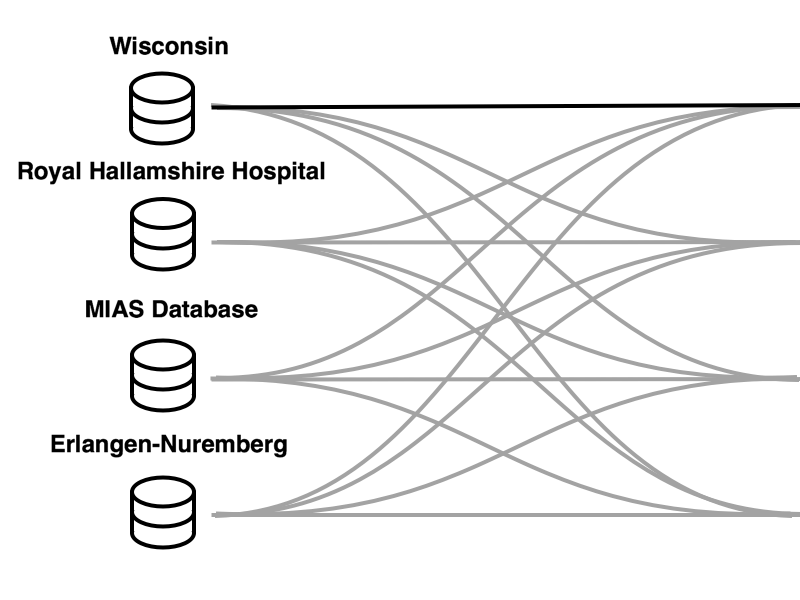
\includegraphics[width=.45\textwidth]{images/KexDbasbild2PNG.png}
    \pause
    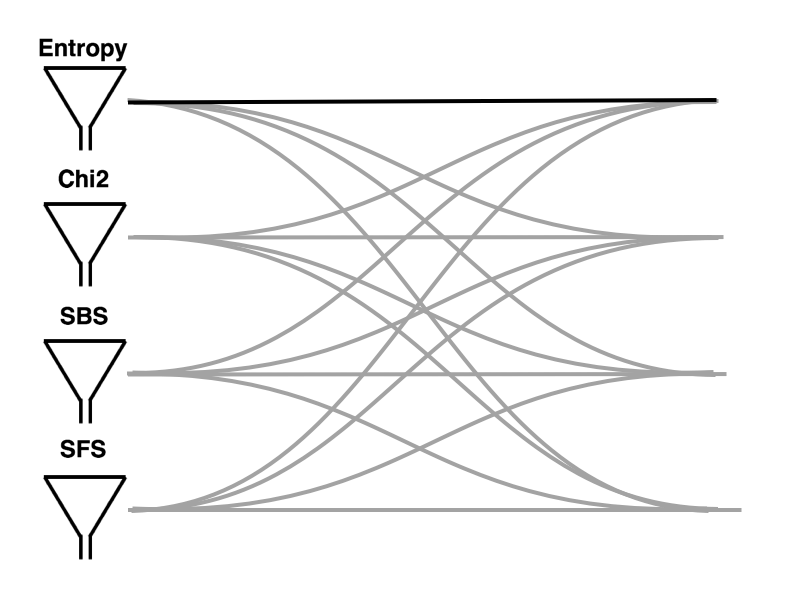
\includegraphics[width=.41\textwidth]{images/KexFilterBildPNG.png}\pause
    
\includegraphics[width=.36\textwidth]{images/kexMLCbildPNG.png}\pause
    }
  \end{figure}
  A total of 800 combinations is calculated
\end{frame}

% ---------- WHAT ----------

\begin{frame}
  \frametitle{\hfill Classification improvements}

    \centering
    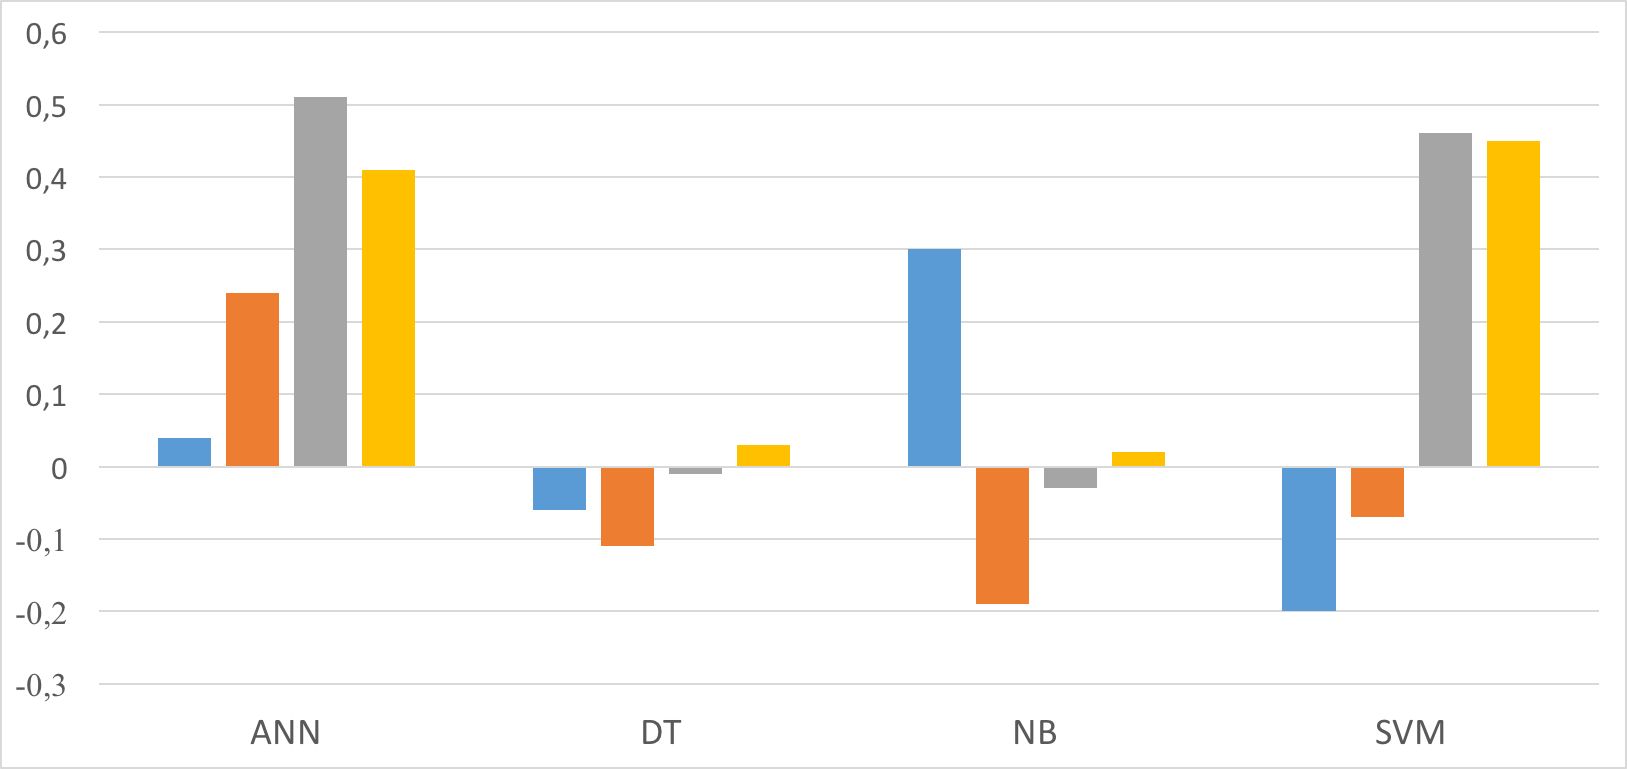
\includegraphics[width=\textwidth]{images/accuracy_improv.png}\\
    Caption
\end{frame}

\begin{frame}
  \frametitle{\hfill ANN's accuracy increase is significant}

  Performing a students t- test we found the accuracy increase of ANN is significant.

  The changes in the other classifiers can not be concluded with statistical significance.
\end{frame}

\begin{frame}
  \frametitle{\hfill 2-way ANOVA}

  2-way ANOVA show the accuracy is dependent on the interaction between chosen FS method and classifier.

  (Insert ANOVA image here)
\end{frame}

\begin{frame}
  \frametitle{\hfill Tukey's test}
  Significant difference among wrappers and filters
\end{frame}

\begin{frame}
  \frametitle{\hfill Conclusion}
  These results allows us to conclude (repeat results from earlier slide here)
  % Put result into a larger context here too
\end{frame}

\begin{frame}
  \frametitle{\hfill }
  Thank you for listening
\end{frame}




\begin{frame}
  \frametitle{\hfill Making a KTH Presentation (Example slide)}

  \begin{block}{Steps needed}
    \begin{itemize}
    \item Copy the following files:
    \begin{itemize}
    \item \texttt{examplepresentation.tex} (this file)
    \item \texttt{beamerthemeKTH.sty}
    \item \texttt{kthgraphics} (with all its contents)
    \end{itemize}
    \item Replace the contents in \texttt{examplepresentation.tex} with your own
    \item Run \texttt{pdflatex} a couple of times
    \item Present your slides using a PDF-viewer
    \end{itemize}
  \end{block}

\end{frame}


\end{document}
